\chapter{Introduction}
\label{ch:introduction}

This thesis covers several problems in mathematical optimization and learning theory.
Optimization is a vast field which plays a crucial role in the technological progress throughout the history.
It was first formalized as a separate subfield at the intersection of mathematics and theoretical computer science in the 20\(^\text{th}\) century, and since then stays an incredibly active area of research.
The main driver for the development of mathematical optimization back then were practical problems in operational research, such as logistics and resource allocation.
Nowadays, optimization methods are the bedrock of the rapid advances in modern machine learning. 

Learning theory studies when is it possible to learn from the data, and what is the most optimal way to do so.
It provides a theoretial foundation behind the machine learning algorithms and lies at the intersection of mathematics, statistics, and theoretical computer science.

It is well-known that there exist optimization problems that are fundamentally difficult to solve.
As an example, finding the largest clique of a graph is a prototipical problem considered to be \emph{hard}, formally defined via \emph{NP-hardness} \dd{add citation, KARP}.
Also, intuitively and somewhat orthogonally, the more parameters the optimization problem has (the larger the optimization space is), the harder it is to optimize over them.
However, as it turns out if the optimization problem is \textit{random}, 
and optimization space is high-dimensional, it becomes possible to argue about the optimal solutions and prove that efficient algorithms can achieve or approximate them.
This is also known as \emph{blessings of dimensionality}, the phenomenon closely studied by high-dimensional probability and modern theoretical computer science.

First part of the thesis is devoted to two different optimization problems and is guided by the following questions:
\begin{enumerate}
  \item Can we solve the optimization problem efficiently?
  \item How well can we approximate a hard optimization problem with an efficient algorithm?
  \item What are the properties of the optimal or approximate solution?
\end{enumerate}
\noindent
Second part of the thesis covers two problems in learning theory under the assumption and all or part of data is \emph{worst-case}, i.e., 
is picked in a worst possible (adversarial) way.

% In the second part of the thesis, we discuss a problem of \emph{Mixture learning} under the presence of adversarial data.

The thesis is organized as follows. 
The remaining part of this chapter contains a brief introduction to the topics discussed in the thesis.
\dd{Add Chapter} discusses the random hitting set problem and the possible greedy heuristics.
In \dd{Add Chapter} we study a classical graph problem of estimating the Lovász number, and bound its expected value over a class of highly structured graphs.
% \dd{Add Chapter} is devoted to the optimization problem in deep learning, namely to the random feature model.
The second part of the thesis, \dd{add Chapter} presents the robust mixture learning problem.
Finally, \dd{add Chapter} presents several open problems which arose during my PhD together with the discussion.
% Correctly treating data with contains outliers is a classical topic, which was initiated by \dd{add citation}.
% Recently, a lot of attention is focus on developing efficient algorithms which work with high-dimensional data.
% Following this line of work, we prove a novel result in robust mixture learning.

% Concretely, we see on the example of classical TCS problem, \(\hs\), 
% which provably cannot be solved efficiently, that when the feasible set of solutions is random, 
% a simple algortihms start to perform much better than what is expected from the worst-case analysis.

% Next, also a classical graph problem of computing Lovász number is studied. 


% Optimization is a fundamental problem, which follows the history of humanity in the form of resource allocation, construction, and trading.
% A basic question that optimization aims to solve is the following:
% \begin{center}
% Given a \textit{feasible set} of solutions and an optimization \textit{objective}, what is the optimal value of the objective?
% \end{center}
% Sometimes we refer to the feasible set as the constraint set, and to the objective as the cost function.
% If the feasible set is obtained by intersection of linear constraints (i.e., halfspaces), and the objective is linear, 
% it is a well-known setting of \textit{linear optimization}. 
% Linear optimization was developed in the 20th century, when breakthrough algorithms, such as simplex and ellipsoid method were developed.
% Recently, with the advance of machine learning field, the non-linear optimization plays an increasingly large role. 

% We refer to the pair of feasible solution set and objective as a problem instance, 
% and the problem is meant as a set of problem instances. 
% As an example, consider the \textit{vertex cover} problem:
% Given a graph \(G = (V, E)\), the goal is to find a smallest set \(S\) of vertices, 
% such that each edge has at least one of its endpoints in \(S\). 
% Our feasible set of solutions are all possible vertex covers for a given graph, 
% and the objective is the size of the vertex cover; the goal is to minimize the objective. 
% For given \(n\), it is straightforward to construct examples where the size of the vertex cover must be \(n / 2\).
% Indeed, if the graph is a perfect matching, then each edge must have a distint vertex covering it.
% Such examples are commonly referred as worst-case examples.
% Furthermore, the vertex cover problem is a classical example of an NP-hard problem, 
% which implies that there is no efficient algorithm that finds an optimal solution.
% A celebrated greedy algorithm can solve vertex cover with a factor 2 approximation.

% In contrast to worst-case examples, there exists a random-case analysis of a problem.
% A probability distribution is imposed on the problem, which can make worst-case problem instances to be exponentially unlikely.
% Here, one of the quantities of interest is the expected behavior of the algorithm given the probability distribution.
% In the context of a vertex cover problem, a classical example would be an Erdős-Rényi random graph model.

% One of the aims of this thesis is to study on a several examples how the randomness assumptions affect the optimization problems.
% In~\Cref{sec:greedy}, we look at the hypergraph version of the vertex cover problem. 
% We study the relation between the optimal value, the linear relaxation, and the algorithmic solution.
% One of our goals is to bound the performance of the greedy algorithm. 
% Recall that the greedy algorithm is a purely deterministic algorithm.
% We proceed by studying a randomized version, called BlockGreedy, and by connecting the performance of the algorithms to each other.
% In~\Cref{sec:lovasz}, we study a problem of bla.
% In~bla, we study a random feature model.

% As another example, where the inputs are sampled from a random distribution, but have some structure, 
% we study the problem of robust mixture learning in~\Cref{chap:robust}.

% Next, we give a brief introduction to the topics studied in this thesis.


\section{Greedy algorithms for the random hitting set problem}
\subsection{Hitting set}

$\hs$ is a classical problem in combinatorial optimization which, for a given ground set $\mathcal{X}\coloneqq\set{1,...,n}$ and a collection $\mathcal{C} \coloneqq \set{\mathcal{S}_1,...,\mathcal{S}_m}$ of subsets of $\mathcal{X}$, asks to identify the smallest set $\mathcal{S}\subseteq \mathcal{X}$ that intersects every subset in $\mathcal{C}$. 
$\hs$ arises naturally from the study of \emph{Minimum Vertex Covers on Hypergraphs} ($\mvch$), upon viewing hyperedges as subsets and vertices as elements of the ground set. 
This is also known as the \emph{Set Cover} problem \cite{paschos1997survey}, which has a rich history in worst-case computational complexity theory, including appearing as one of Karp's 21 NP-complete problems. 
An important question regards the behaviour of natural random instances of $\hs$ where each element of the ground set is independently assigned to any subset with probability $p$.
Such problem formulation is motivated, among others, by applications such as group testing \cite{iliopoulos2021group}. 
A classical theorem of Lovász \cite{lovasz1975ratio} gives an upper bound on the integrality gap in this problem which grows with the degree of the underlying hypergraph, i.e., the maximum number of subsets intersecting any one element. 
This bound was shown to be tight in the worst-case, but leaves much to be desired from an average-case perspective.

In this chapter, we characterize the average-case integrality gap present in random $\hs$ and prove that, with high probability, Lovász's greedy algorithm \cite{lovasz1975ratio} finds the minimal (up to a multiplicative constant) hitting set in polynomial time. 

\subsection{Random integer and linear programs}
We consider the following integer programming ($\ip$) formulation of the problem,
\begin{equation}
\label{def:ip}
\valip:=  
\begin{cases}
\begin{aligned}
& \min_{x \in \R^n}
& & \norm{\x}_1 \\
& \text{subject to}
& &  \A\x \geq \mathbf{1} , \: \x \in \set{0,1}^n,
\end{aligned}
\end{cases}
\end{equation}
where the $i$-th row of $\A \in \set{0,1}^{m\times n}$ provides a binary encoding of the membership of the elements of $\mathcal{X}$ in the set $\mathcal{S}_i$ and $\mathbf{1} := (1, \ldots, 1) \in \mathbb{R}^m$. With the vertex cover formulation of the problem at hand, we note that $\A$ consists of the incidence matrix of the underlying hypergraph.
In particular, the constraint \(\A\x \geq \mathbf{1}\) ensures that each set in $\mathcal{C}$ is hit by a prescribed candidate solution vector. A natural convex relaxation is obtained by allowing fractional solutions, and may be expressed as the following linear program ($\lp$),
\begin{equation}
\label{def:lp}
\vallp:=
\begin{cases}
\begin{aligned}
& \underset{\x}{\text{minimize}}
& & \norm{\x}_1 \\
& \text{subject to}
& & \A\x \geq \mathbf{1}, \:  \x \in [0,1]^n.
\end{aligned}
\end{cases}
\end{equation}
Whilst clearly $\vallp\leq \valip$, tightness need not hold in general. In fact, for $m = n$ and $\A \in \set{0,1}^{n\times n}$ chosen such that each row and column contains exactly $k$ ones, for some fixed $1 < k < n$, an optimal solution is provided by $\x^*_{\texttt{LP}}=\left(1/k,...,1/k\right)$, which is not integral, thus leading to a strictly smaller objective whenever $n / k$ is not an integer. This evidences the existence of a multiplicative \emph{integrality gap}, as we define next.
\begin{definition}
    Given solutions \(\valip\) and \(\vallp\) to~\Cref{def:ip} and~\Cref{def:lp} respectively, we define \emph{multiplicative integrality gap} as follows:
    \begin{equation}
        \ipgap \coloneqq \frac{\valip}{\vallp}.
    \end{equation}
\end{definition}
In \cite{lovasz1975ratio}, Lovász proved an essentially optimal worst-case upper bound on the $\hs$ multiplicative integrality gap: $\ipgap \leq 1+\log \dmax$, where $\dmax$ corresponds to the maximum degree in the underlying hypergraph. 
This is obtained by analysing the \greedy algorithm (Algorithm~\ref{alg:greedy}), 
which constructs a vertex cover by sequentially adding vertices with the highest degree amongst the uncovered edges, 
and will be discussed in more detail in the next sections \dd{in Chapter Bla}. 
However, in many natural examples, the maximum degree $\dmax$ grows with the number of vertices in the hypergraph, thus leading to progressively worse bounds for increasingly large hypergraphs. Besides being arguably the most natural candidate for solving $\hs$, the greedy algorithm has been shown to be the best possible polynomial time approximation algorithm \cite{slavik1996tight} for the worst-case instances of this classical problem. 

Despite extensive work conducted on $\hs$ in the last decades, a gap remains in our understanding of the typical performance of linear programming and the greedy algorithm on random problem instances. 
We hence pose the following questions: 

\begin{enumerate}
    \item Are there integrality gaps in random instances of $\hs$? 
    \item Can near-optimal solutions be found efficiently? 
\end{enumerate}

\noindent
In the present work \dd{add Chapter}, we provide answers to the above questions 
\emph{with high probability} (w.h.p.) in a non-asymptotic sense, 
in the setting where the cardinality $n$ of the ground set $\mathcal{X}$ 
is large but finite. 
We prove the absence of integrality gaps up to constants in a wide regime of $n,m,p$, by conducting an average case analysis of an algorithm that outputs integral covers of matching size to the fractional ones. 
In addition, a rigorous analysis of the greedy routine will follow by a straightforward reduction. 

\subsection{Greedy algorithm}

\begin{algorithm}[!t]
    \caption{\greedy}\label{alg:greedy}
    \begin{algorithmic}[1]
    \State \(\mathcal{I} \gets \{I_1, \ldots, I_n\} \) \Comment{Inclusion sets}
    \State \(U \gets [m]\)
    \State \(t \gets 0\)
    \While{\(|U| > 0\)}
        \State \(P \gets \mathrm{argmax}_{I \in \mathcal{I}}\bigl|I \cap U\bigr| \) \Comment{Greedy step}
        \State \(\mathcal{I} \gets \mathcal{I} \setminus \{P\}\)
        \State \(U \gets U \setminus P\)
        \State \(t \gets t + 1\)
    \EndWhile
    \State \(\valgr \gets t\)
    \State \Return \(\valgr\)
    \end{algorithmic}
    \end{algorithm}

The core principle of \greedy,~\Cref{alg:greedy}, is to construct a feasible solution in steps, by sequentially adding to the candidate solution an element which hits the largest number of remaining sets. 
In the chosen setting, where elements are added to sets with equal probability and independently of each other, we have precise estimates on the number of subsets hit by an element which is {\it picked first}. 
In fact, the size of this set is given by the maximum of independent Binomial random variables, which is analysed in \Cref{sec:bounds}. 
However, this very first step introduces nontrivial dependencies amongst the remaining matrix columns and significantly complicates keeping track of the marginal gains of each subsequent element addition to the candidate solution.




In order to circumvent this issue, we introduce a modified greedy routine, which we refer to as the \bgreedy\ algorithm, where the elements of the ground set $[n]$ are split into separate sets of a given size, which we call blocks. 
At the \(t\)-th iteration, the algorithm picks the element hitting the largest number of remaining sets across \textit{the first} \(t\) \textit{blocks only}. 
By choosing the size of the blocks appropriately, we have that at each iteration $t$ one is guaranteed to find a solution of near-optimal size within the set of newly-included independent columns. 

\noindent

\bgreedy is detailed in Algorithm~\ref{alg:block_greedy}, whilst informally, it works as follows.
\begin{enumerate}
\item Let \(K\) be the size of the solution (suggested by theoretical analysis);
\item Uniformly at random split \(n\) columns into \(K\) blocks with \(n / K\) columns per block;
\item Start with an empty set of possible choices of columns;
\item At the \(t\)-th iteration, first add the columns
from the \(t\)-th block (Step~\ref{step:adding_new_block} \dd{Fix reference here and next}).
Then, perform one greedy step on the current
set of possible choices (Step~\ref{step:greedy_step});
\item If after \(K\) iterations of the algorithm, some subsets remain uncovered, we use  a trivial covering, i.e., covering each subset by a separate column.
\end{enumerate}
Note that the first selection of the element which hits the most number of subsets again introduces dependencies. 
However, the columns that are in the newly added block are independent of everything else at time \(t\).

\begin{figure}[!t]
    \centering
  \begin{tikzpicture}
    \begin{axis}[ymin = 0, ymax = 0.45, axis lines=middle, height=6cm, width=10cm,
    legend style={
      at={(1,1)}
      },
    axis line style={->},
    x label style={at={(axis description cs:0.96,-0.14)},anchor=south},
    y label style={at={(axis description cs:-0.05,0.9)},anchor=south},
    xlabel={\large $m(n)$},
    ylabel={\large $p(n)$},
    xtick={1.58, 3.98, 10, 25.11},
    xticklabels={ $n^{0.1}$,
                 $n^{0.3}$,
                 $n^{0.5}$, 
                 $n^{0.7}$},
    ytick={0.01,0.039,0.1,0.25,0.63},
    yticklabels={ $1 / n^{0.9}$,
                 $1 / n^{0.7}$,
                 $1 / n^{0.5}$,
                 $1 / n^{0.3}$,
                 $1 / n^{0.1}$},]
        \addplot[thick, color=red, smooth, name path = inv, domain = 1:40, line width=2pt] {1.5/x};
        \addplot[name path = floor, draw = none] coordinates {(1,0) (40,0)};
        \addplot[fill=red, 
        fill opacity=0.2] fill between[of = inv and floor];
        \path[name path=axis] (axis cs:0,40) -- (axis cs:40,40);
        \addplot[fill = blue, fill opacity=0.3] fill between[of= inv and axis];
        \legend{\large $ mp \sim \log n$}
    \node[below, text=red!30!black,font=\bfseries] at (15, 0.06) {\valbgr \(\sim\) \valip \(\sim\) \vallp \(\sim m / \dmax\)};
    \node[above, text=blue!80!black, font=\bfseries] at (20,0.2) {\valbgr \(\sim\) \valip \(\sim \log\left(\frac{mp}{\log n}\right) / p \)};
    \node[above, text=blue!80!black, font=\bfseries] at (22, 0.13) {\vallp \(\sim 1/p\)};
\end{axis}
\end{tikzpicture}
\caption{Transition between the sparse and the dense regime for different values of the average inclusion set size $mp$.}
    \label{fig:phase_diagram}
\end{figure}

\subsection{Main contributions}

Given a collection of sets \(\mathcal{C} := \set{\mathcal{S}_1,...,\mathcal{S}_m}\), we define inclusion sets $I_j := \set{i \in [m]\: : \: j \in \mathcal{S}_i}$, for $j \in [n]$, which in the \(\mvch\) formulation of the problem at hand correspond to the set of hyperedges incident to any given vertex. 
Furthermore, we let \(\dmax \coloneqq \max_{j \in [n]} \card{I_j}\). 
Throughout, we use the notation $\text{val}_{\mathtt{Gr}}$, $\valbgr$ to denote the size of the hitting set returned by $\greedy$ and $\bgreedy$ respectively. 
Below we provide an informal description of the main results (also shown in~\Cref{fig:phase_diagram}) which hold with high probability, 
where $A(n) \sim B(n)$ denotes that $c A(n) \leq B(n) \leq C A(n)$ for large enough $n$ and for some constants $c, C > 0$: 
\paragraph*{\textbf{Sparse Regime} ($mp \ll \log n$):}
We show that \(\ipgap \sim 1\) in the sparse regime by proving that the \bgreedy algorithm succeeds in reaching the \lp lower bound of $\frac{m}{\dmax}$.
\[ \valbgr \sim \valip \sim \vallp \sim \frac{m}{\dmax}. \]

% \vspace{0.3em}

\paragraph*{\textbf{Dense Regime} ($mp \gg \log n$):}
We prove that \(\ipgap \sim \log \frac{mp}{\log n}\) in the dense regime. We show that the \bgreedy algorithm performs as well as \ip in this regime, i.e.
\[ \frac{1}{p} \log\left(\frac{mp}{\log n}\right) \sim \valbgr \sim \valip \gg \vallp \sim \frac{1}{p} \sim \frac{m}{\dmax}. \] 

% \vspace{0.3em}

\paragraph*{\textbf{Threshold Regime} ($mp \sim \log n$):} This regime smoothly interpolates between the sparse and dense ones, with \(\ipgap \sim 1\). 
The scaling for all quantities of interest is $m / \dmax \sim 1/p$.

% \vspace{0.3em}

\paragraph*{\textbf{Greedy}:} We prove that $\valgr \sim \valip$ when $\frac{\log 1 / p}{\log n} < 1/2$. 



\section{Lovász number for random circulant graphs}

\subsection{Lovász number}

\begin{figure}[t!]
    \centering
    \begin{tabular}{cc}
    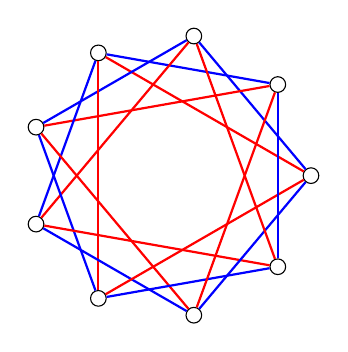
\begin{tikzpicture}[scale=1.2]
      \foreach \i in {0,...,8} {
        \node[draw, circle, inner sep=2pt] (v\i) at ({360/9 * \i}:1.5cm) {};
      }
      \foreach \i in {0,...,8} {
        \pgfmathtruncatemacro{\nextTwo}{mod(\i+2,9)}
        \draw[blue, thick] (v\i) -- (v\nextTwo);
        \pgfmathtruncatemacro{\nextThree}{mod(\i+3,9)}
        \draw[red, thick] (v\i) -- (v\nextThree);
      }
    \end{tikzpicture}
    &
    
    \begin{tikzpicture}[every node/.style={minimum size=0.3cm, anchor=center, font=\footnotesize}, scale=0.6]
    \matrix (m3) [matrix of nodes,
        left delimiter={(},
        right delimiter={)},
        row sep=-\pgflinewidth, column sep=-\pgflinewidth
    ]{
      $\cdot$ & $\cdot$ & $\textcolor{blue}{\mathbf{1}}$ & $\textcolor{red}{\mathbf{1}}$ & $\cdot$ & $\cdot$ & $\textcolor{red}{\mathbf{1}}$ & $\textcolor{blue}{\mathbf{1}}$ & $\cdot$ \\
      $\cdot$ & $\cdot$ & $\cdot$ & $\textcolor{blue}{\mathbf{1}}$ & $\textcolor{red}{\mathbf{1}}$ & $\cdot$ & $\cdot$ & $\textcolor{red}{\mathbf{1}}$ & $\textcolor{blue}{\mathbf{1}}$ \\
      $\textcolor{blue}{\mathbf{1}}$ & $\cdot$ & $\cdot$ & $\cdot$ & $\textcolor{blue}{\mathbf{1}}$ & $\textcolor{red}{\mathbf{1}}$ & $\cdot$ & $\cdot$ & $\textcolor{red}{\mathbf{1}}$ \\
      $\textcolor{red}{\mathbf{1}}$ & $\textcolor{blue}{\mathbf{1}}$ & $\cdot$ & $\cdot$ & $\cdot$ & $\textcolor{blue}{\mathbf{1}}$ & $\textcolor{red}{\mathbf{1}}$ & $\cdot$ & $\cdot$ \\
      $\cdot$ & $\textcolor{red}{\mathbf{1}}$ & $\textcolor{blue}{\mathbf{1}}$ & $\cdot$ & $\cdot$ & $\cdot$ & $\textcolor{blue}{\mathbf{1}}$ & $\textcolor{red}{\mathbf{1}}$ & $\cdot$ \\
      $\cdot$ & $\cdot$ & $\textcolor{red}{\mathbf{1}}$ & $\textcolor{blue}{\mathbf{1}}$ & $\cdot$ & $\cdot$ & $\cdot$ & $\textcolor{blue}{\mathbf{1}}$ & $\textcolor{red}{\mathbf{1}}$ \\
      $\textcolor{red}{\mathbf{1}}$ & $\cdot$ & $\cdot$ & $\textcolor{red}{\mathbf{1}}$ & $\textcolor{blue}{\mathbf{1}}$ & $\cdot$ & $\cdot$ & $\cdot$ & $\textcolor{blue}{\mathbf{1}}$ \\
      $\textcolor{blue}{\mathbf{1}}$ & $\textcolor{red}{\mathbf{1}}$ & $\cdot$ & $\cdot$ & $\textcolor{red}{\mathbf{1}}$ & $\textcolor{blue}{\mathbf{1}}$ & $\cdot$ & $\cdot$ & $\cdot$ \\
      $\cdot$ & $\textcolor{blue}{\mathbf{1}}$ & $\textcolor{red}{\mathbf{1}}$ & $\cdot$ & $\cdot$ & $\textcolor{red}{\mathbf{1}}$ & $\textcolor{blue}{\mathbf{1}}$ & $\cdot$ & $\cdot$ \\
    };
    \end{tikzpicture}
    \\[0.0em]
    \end{tabular}
    \caption{Circulant graph on \(9\) vertices and its adjacency matrix (0's replaced by dots). Each vertex \(i\)  is connected to vertices \(\textcolor{blue}{i \pm 2}\) and \(\textcolor{red}{i \pm 3} \mod 9\).}
    \label{fig:circ_graphs}
    \end{figure}

The Lovász number $\vartheta$ is a well-known statistic of an arbitrary simple undirected graph $G$. 
As Lovász first observed in \cite{lovasz1979shannon}, one can define a number $\ltn(G)$ 
as the value of a certain semidefinite program (SDP) 
whose constraints depend on the adjacency matrix of $G$.
The Lovász number provides an upper bound on the Shannon capacity of the graph and satisfies the following inequalities:
\begin{equation}
\label{eq:theta_ineq}
\omega(G) \leq \ltn(\overline{G}) \leq \chi(G),
\end{equation}
where $\omega(G)$ is the size of the largest clique in $G$, $\chi(G)$ is the chromatic number of $G$, and $\overline{G}$ is the complement of $G$. 
This observation is remarkable, since $\vartheta$ is computable in polynomial time, while $\omega$ and $\chi$ are famously NP-hard to compute. 

The Lovász number has been studied for a variety of random graph models including the classical Erd\H{o}s-R\'{e}nyi (ER) random graph $G(n, p)$. 
Its expected value was first studied by Juh{\'a}sz~\cite{juhasz1982asymptotic}, 
who showed that $\E \ltn(G) = \Theta(\sqrt{n/p})$ for $\frac{\log^6 n}{n} \le p \le 1/2$. 
For $p=1/2$, Arora and Bhaskara~\cite{aroranote} showed that \(\ltn(G)\) concentrates around its median in an interval of polylogarithmic length.
In the sparse regime $p < n^{-1/2}$, it has been further shown that \(\ltn(G)\) concentrates around its median in an interval of constant length~\cite{coja2005lovasz}.
To the best of our knowledge, determining the correct constant in the $\Theta(\sqrt{n/p})$ asymptotic remains an open question. 

\subsection{Random circulant graphs}
In this chapter, we focus on a class of random \emph{circulant} graphs (RCGs), a family of vertex-transitive graphs with a circulant adjacency matrix; see~\Cref{fig:circ_graphs} and~\Cref{def:circ_graph,def:rand_circ} \dd{Why theorems, not definitions???}. 
We emphasize that RCGs are fully determined by the connectivity of any given single vertex. Therefore, a dense RCG can be generated with \(\frac{n - 1}{2}\) random bits, where each bit affects the presence of \(n\) edges, in contrast to the \(\frac{n(n - 1)}{2}\) random bits in $G(n,1/2)$, each affecting just one edge.
In this sense, RCGs may be viewed as a ``partial derandomization'' of ER graphs.
Indeed, circulant graphs are precisely Cayley graphs on the group \(\mathbb{Z}_n\), and general random Cayley graphs have long been studied for similar purposes in theoretical computer science.


It is therefore of interest to understand to what extent the above results for ER graphs also apply to RCGs.
For dense RCGs, the asymptotics of the clique number and the chromatic number are well-understood:~\cite{green2005counting} showed a high-probability upper bound on the clique number \(\omega(G) = O(\log n)\), and later~\cite{green2016counting} proved that the chromatic number is at most $(1+o(1)) \frac{n} { 2 \log_2 n}$ with high probability. 
These results imply bounds on the Lovász number through~\Cref{eq:theta_ineq}, but the resulting upper and lower bounds are far apart.

Our main result is much sharper upper and lower bounds on the expected Lovász number of a dense RCG. 
\begin{theorem}
\label{thm:main}
    There exists a constant $C > 0$ such that, for a dense random circulant graph \(G\) on $n$ vertices (\Cref{def:rand_circ}),
    \begin{equation}
        \sqrt{n} \leq \E \ltn(G) \leq C \sqrt{n \log \log n}.
    \end{equation}
\end{theorem}

\noindent

\subsection{Proof strategy}
Our proof of the upper bound in~\Cref{thm:main} relies on the algebraic structure of circulant graphs. First, following~\cite{magsino2019linear}, we transform the SDP formulation of \(\ltn(G)\) to a linear program (LP) using the fact that the circulant matrices are diagonalizable by a discrete Fourier transform (DFT)
\Cref{lem:lp_with_g} gives the resulting LP:
\begin{equation}
\label{eq:first_step}
\begin{aligned}
    \ltn(G) &= \max_{(y_0, \dots, y_{n-1}) \in \R^{n}} \braket{y, g}, \\ \text{ subject to }
    &\begin{cases} y_k = y_{n - k} \text{ for } k = 1,\ldots, n - 1, \\
    \norm{y}_1 = 1,
    y \geq \mathbf{0}, \\
    \braket{y, f_k} = 0\text{ for all edges } (0, k).
    \end{cases}
\end{aligned}
\end{equation}
Here, \(f_k\) is the \(k\)-th row of the DFT matrix \(F\), and \(g \coloneqq Fb\) for \(b \in \{\pm 1\}^{n}\) with $b_0=1$ and \(b_k = 1\) if \((0, k)\) is not an edge, and \(-1\) otherwise, for $1 \le k \le n-1$. We denote \(\mathbf{0} \coloneqq (0, \ldots, 0)\) and \(y \geq \mathbf{0}\) stands for entrywise positivity of \(y\).

The last constraint in~\Cref{eq:first_step} requires the Fourier transform of \(y\) to have a specific sparsity pattern. Uncertainty principles for the Fourier transform (see, e.g.,~\cite{bandeira2018discrete}) then suggest that all feasible vectors \(y\) must be dense \cite{demanet2014scaling}.
A quantitative version of this ``density'' would be enough to bound the LP.
To illustrate, suppose that $y$ is a feasible vector with $\|y\|_1 = 1$ and its mass is spread almost uniformly among its coordinates, i.e., that
\(\norm{y}_2 \leq \frac{c}{\sqrt{n}} \norm{y}_1 = \frac{c}{\sqrt{n}}\), for some constant \(c > 0\). Since \(\norm{g}_2 = n\), Cauchy-Schwarz inequality would give \(\braket{y, g} \leq \norm{y}_2 \norm{g}_2 \leq c\sqrt{n},\) proving upper bound in~\Cref{thm:main} without the extra \(\sqrt{\log \log n}\) factor.

The second part of our proof,~\Cref{lem:rip}, makes the aforementioned intuition rigorous, relying on the \textit{restricted isometry property} (RIP,~\Cref{def:rip}).
The $f_k$ in our constraints form a so-called \emph{subsampled DFT basis}, which is a random subset of the Fourier basis.
The RIP for such bases is in fact a celebrated topic in the compressed sensing literature. RIP was first introduced and studied for subsampled DFT bases in seminal work of Candès and Tao~\cite{candes2006near},
and since then, one of the central 
questions for compressed sensing is 
the number of $f_k$ needed for RIP to hold. 
\Cref{lem:rip_dft} describes a simplified version of the current best bound due to~\cite{haviv2017restricted} which is sufficient for our purposes.
Interestingly, our upper bound proof only uses the fact that feasible solutions of~\Cref{eq:first_step} lie on a (random) nullspace of a subsampled DFT matrix, and omits the positivity constraint \(y \geq \mathbf{0}\). However, as we discuss in~\Cref{sec:discussion}, we believe that this constraint is important for tighter results.


% \section{Deep random feature model}
% \input{chapters/introduction/content/deeprf}
% \subsection{High-dimensional regression}
% \subsection{Random matrix theory}
% \subsection{Random feature model}

\section{Lower bounds for online private learning}
\glsresetall
With the increasing need to protect the privacy of sensitive user data while conducting meaningful data analysis,~\Gls{dp}~\citep{dwork2006calibrating} has become a popular solution.~\Gls{dp} algorithms ensure that the impact of any single data sample on the output is limited, thus safeguarding individual privacy. Several works have obtained~\Gls{dp} learning algorithms for various learning problems in both theory and practice.

However, privacy does not come for free and often leads to a statistical (and sometimes computational) cost. 
The classical solution for non-private~\Gls{pac} learning~\citep{valiant1984theory} is via~\Gls{erm} that computes the best solution on the training data. Several works~\citep{bassily2014private,chaudhuri2011differentially} have shown that incorporating DP into~\Gls{erm} incurs a compulsory statistical cost that depends on the dimension of the problem. In the well-known setting of~\Gls{pac} learning with~\Gls{dp},~\citet{kasiviswanathan2011can} provided the first guarantees that all finite VC classes can be learned with a sample size that grows logarithmically in the size of the class. This line of research was advanced by subsequent works~\citep{beimel2013characterizing,feldman2014sample,beimel2014bounds}, resulting in the findings of~\citet{alon2022private} which established a surprising equivalence between non-private online learning and~Approximate~\Gls{dp}-\Gls{pac} learning.

Unlike the setting of~\Gls{pac} learning, Online learning captures a sequential game between a learner and an adversary. 
The adversary knows everything about the learner's algorithm except its random bits. 
In this work we consider a setting where, for a known hypothesis class \(\hyp\), the adversary chooses a sequence of data points \(\bc{x_1,\ldots,x_t}\) and the target hypothesis \(f^*\in\hyp\) prior to engaging with the learner. Then, the adversary reveals these data points one by one to the learner, who must offer a prediction for each. After each prediction, the adversary reveals the true label for that point. The learner's performance is evaluated by comparing the incurred mistakes against the theoretical minimum that could have been achieved by an optimal hypothesis in hindsight. Known as the \emph{realisable oblivious mistake bound} model, the seminal work of~\citet{littlestone1988learning} showed that i) the number of mistakes incurred by any learner is lower-bounded by the Littlestone dimension~(more precisely, \(\nicefrac{\ldim{\hyp}}{2}\)) of the target class \(\hyp\) and ii) there is an algorithm that makes at most~\(\ldim{\hyp}\) mistakes. This algorithm is commonly referred to as the~\Gls{soa}.

Recall that certain problem classes possess finite Vapnik-Chervonenkis (VC) dimensions but infinite Littlestone dimensions (such as the one-dimensional threshold problem). 
This, together with the equivalence between non-private online learning and ~\Gls{dp}-\Gls{pac} learning~\citep{alon2022private} implies that there exists a fundamental separation between DP-PAC learning and non-private PAC learning. In other words, some learning problems can be solved with vanishing error, as the amount of data increases, in~\Gls{pac} learning but will suffer unbounded error in~\Gls{dp}-\Gls{pac} learning. This implication was first proven for pure~\Gls{dp} by~\citet{feldman2014sample} and later for approximate~\Gls{dp} by~\citet{alon2019private}. With the debate on the sample complexity of approximate~\Gls{dp}-\Gls{pac} learning resolved, we next ask whether a similar gap exists between online learning with~\Gls{dp} and non-private online learning.~\citet{golowich2021littlestone} addressed this by introducing the~\Gls{dpsoa}, which suffers a mistake count, that increases logarithmically with the number of rounds \(T\) compared to a constant error rate in non-private online learning~\citep{littlestone1988learning}. This difference suggests a challenge in~\Gls{dp} online learning, where errors increase indefinitely as the game continues. The question of whether this growing error rate is an unavoidable aspect of DP-online learning was posed as an open question by~\citet{dpopsanyal22a}.

\paragraph{Main Result} In this work, we provide evidence that this additional cost is inevitable. Consider any hypothesis class \(\cH\) and for a learning algorithm \(\alg\). Let \(\bE\bs{\regret_{\alg}}\) be the expected number of mistakes incurred by \(\alg\) and let \(T\) be the total number of rounds for which the game is played. 


We obtain a lower bound on \(\bE\bs{M_{\cA}}\) under some assumptions on the learning algorithm \(\cA\). Informally, we say an algorithm \(\cA\) is \(\conc{\beta}\)~(see~\Cref{defn:beta-conc} for a formal definition) if there is some output sequence that it outputs with probability at least \(1-\beta\) in response to a~\emph{non-distinguishing} input sequence. A~\emph{non-distinguishing} input sequence is a~(possibly repeated) sequence of input data points such that there exists some \(f_1,f_2\in\hyp\) which cannot be distinguished just by observing their output on the non-distinguishing input sequence. We prove a general statement for any hypothesis class in~\Cref{thm:main-finite} but show a informal corollary below.

\begin{corollary}[Informal Corollary of~\Cref{thm:main-finite}]\label{thm:informal-small}
     There exists a hypothesis class \(\cH\) with \(\ldim{\cH}=1\) (see~\Cref{defn:littlestone}), such that for any \(\e, \delta > 0, T \leq \exp(1/(32\delta))\), and any online learner \(\alg\) that is \((\e, \delta)\)-\Gls{dp} and \(0.1\)-concentrated, there is an adversary, such that 
    \begin{equation}
        \E\bs{\regret_{\alg}} =\widetilde\Omega\br{\frac{\log T}{\e}},
        \end{equation}
    where \(\widetilde \Omega\) hides logarithmic factors in \(\e\). For \(T > \exp(1/(32\delta))\), \(\E\bs{\regret_{\alg}} = \widetilde\Omega\br{1 / \delta}\).
\end{corollary}

 While the above result uses a hypothesis class of Littlestone dimension one, our main result in~\Cref{sec:finite_horizon_result} also holds for any hypothesis class, even with Littlestone dimension greater than one. Utilising the \(\point_N\) hypothesis class (see~\Cref{defn:point-class}) in~\Cref{thm:informal-small}, we demonstrate that the minimum number of mistakes a~\Gls{dp} online learner must make is bounded below by a term that increases logarithmically with the time horizon \(T\). 
 This holds if the learning algorithm is concentrated and \(T\) is less than or equal to \(\exp\br{1 / (32\delta)}\). This contrasts with non-private online learning, where the number of mistakes does not increase with \(T\) in hypothesis classes with bounded Littlestone dimension, even if the learner is concentrated.\footnote{All deterministic algorithms are \(\conc{0}\) by definition.} Our result also shows that the analysis of the algorithm of~\citet{golowich2021littlestone}, which shows an upper bound of~\(\Omega\br{\log \br{T/\delta}}\) for~\Gls{dpsoa} is tight as long as \(T\leq\exp\br{1 / (32\delta)}\). However, as illustrated in~\Cref{fig:lower-bound}, this is not a limitation as for larger \(T\), since a simple~\emph{Name \& Shame} algorithm incurs lesser mistake than~\Gls{dpsoa} albeit at vacuous privacy levels (see discussion after~\Cref{thm:main-finite}). 


In fact, the assumption of concentrated learners is not overly restrictive given that known~\Gls{dp}-online learning algorithms exhibit this property, as detailed in~\Cref{sec:example-conc}. Notably, the~\Gls{dpsoa} presented by~\citet{golowich2021littlestone} which is the sole DP online learning method known to achieve a mistake bound \(\bigO{\log\br{T}}\), is concentrated as shown in~\Cref{lem:dpsoa-conc}. This suggests that the lower bound holds for all potential~\Gls{dp} online learning algorithms.


Additionally, we extend our result to another class of~\Gls{dp} online algorithms, which we refer to as~\emph{uniform firing} algorithms, that are in essence juxtaposed to concentrated algorithms.  These algorithms initially select predictors at random until a certain
confidence criterion is met, prompting a switch to a consistent predictor—this transition, or `firing', is determined by the flip of a biased coin (with bias \(p_t\)), where the likelihood of firing increases with each mistake. However, the choice of how \(p_t\) increases and the selection of the predictor upon firing depend on the algorithm's design. For this specific type of algorithms, particularly in the context of learning the \(\point_3\) hypothesis class, Proposition~\ref{prop:firing-lb} establishes a lower bound on mistakes that also grows logarithmically with \(T\).


\Cref{sec:continual} discusses Continual Observation~\citep{dwork2010boosting,chan2011private}, another popular task within sequential~\Gls{dp}. We show that results on~\Gls{dp}~Continual Counters can be used to derive upper bounds in the online learning setting. Nonetheless, it is not clear whether lower bounds for that setting can transferred to~\Gls{dp}-Online learning. In addition, these upper bounds suffer a dependence on the hypothesis class size. 

Finally, we point out that, to the best of our knowledge we are unaware of any algorithms in the literature for pure~\Gls{dp} online learning. Our lower bound in~\Cref{thm:informal-small} immediately provides a lower bound for pure~\Gls{dp}. Similarly, DP Continual Counters provide a method for achieving upper bounds, specifically for the \(\point_N\) classes, albeit with a linear dependency on \(N\). Obtaining tight upper and lower bounds remains an interesting direction for future research.


\section{Robust mixture learning}
% Second part of this thesis is devoted to robust statistics, in particular to high-dimensional algorithmtic robust statistics. 

\subsection{Robust mean estimation}
A classical problem in robust statistics is \textit{robust mean estimation}.
It is formulated as follows: 
For a known family of distributions \(\cP\), a learner is provided with a dataset of \(n\) points, where one part comes from a distribution \(P \in \mathcal{P}\), 
while the rest is generated by an adversarial model. 
The task of the learner is to reliably and accurately estimate \(\E_{P} X\), the mean of \(P\).

A few clarifications are in order. 
First, there exist several different adversarial models, some of them listed below.
In what follows, \(\varepsilon \in (0, 1/2)\) denotes the proportion of adversarial points and \(n\) denotes the total dataset size.
\begin{enumerate}
    \item \textit{Strong adversary.} In this model, in the beginning \(n\) samples are generated i.i.d. from \(P\). 
    Adversary removes or replaces up to \(\lceil \varepsilon n \rceil\) of them with arbitrary points.
    The learner then receives the modified dataset.
    \item \textit{Weak adversary.} Here, adversary picks an arbitrary distribution \(Q\).
    The learner receives the dataset of i.i.d. samples from the mixture \((1 - \varepsilon) P + \varepsilon Q\).
    \item \textit{Mean-shift contamination.} For this model, let \(\overline{P}\) denote the centered distribution \(P\).
    The adversary picks \(k \coloneqq \lceil \varepsilon n \rceil\) points \(z_1, \ldots, z_k\).
    The final dataset consists of \(n - k\) i.i.d. samples from \(P\) and the remaining \(k\) points are obtained by sampling \(x_i \overset{\mathrm{i.i.d.}}{\sim} \overline{P}\) and adding \(z_i\) to it.
\end{enumerate}
\noindent
These models are ordered by how restricted the adversary is. Weak adversary model is also known as Huber contamination model.
In all models, adversary has the knowledge of \(\cP\), and of the algorithm which the learner will be using (apart from the internal randomness of the algorithm).

Second, our goal is to design an algorithm for the learner that is computationally efficient in high dimenions.
In particular, its time and sample complexity must be (quasi-)polynomial in the dimension \(d\) of the samples.

Finally, \emph{reliable} estimate means that the guarantees of the algorithm must hold with high probability over the randomness of the sampling procedure and the internal randomness of the algorithm.
\emph{Accurate} estimate means that the error (usually measured as the \(\ell_2\) distance between the estimate and the true parameter)
does not depend on the dimension \(d\).

In one dimensional case, the median is a great candidate for an efficient and robust mean estimator. 
Indeed, when the samples come from \(\cN(\mu, 1)\) in the strong adversary model \dd{how general is this?}, 
it is easy to show that the median \(\muhat\) satisfies \(\norm{\muhat - \mu}_2 = O(\varepsilon)\) with high probability.
From straightforward TV distance arguments, \(O(\varepsilon)\) is the optimal achievable error.

However, computing median in high dimensions is challenging. 
Consider for simplicity the case \(\cP = \set{\cN(\mu, I), \text{ for } \mu \in \R^d}\).
If we compute median coordinate-wise, then the (in general unimprovable) error is \(O(\sqrt{d} \varepsilon)\), 
which is not accurate, since it depends on the dimension \(d\).
There exists another generalization of median to high dimensions, called \textit{Tukey median}, which is defined as follows:
\begin{equation}
    \mu_{\mathrm{Tukey}} \coloneqq \arg \max_{\muhat \in \R^d} \inf_{v \in \R^d} \Pr(v^\top (X - \muhat) \geq 0).
\end{equation}

Tukey median is an accurate estimator: it achieves error \(O(\varepsilon)\) with high probability. 
However, to compute Tukey median is an NP-hard problem, thus it cannot be used as a candidate for an efficient algorithm.

Recent breakthrough results \dd{add citation} show how to achieve error \(O(\varepsilon)\) efficiently.
One of the ideas is a filtering approach.

\subsection{Clustering and list-decodable mean estimation}

\begin{algorithm}[t]
    \caption{K-Means}
    \label{alg:kmeans}
        \begin{algorithmic}[1]
            \Require Samples \(S = \Set{x_1, \ldots, x_{n}}\), number of centers \(k\).
            \Ensure Clusters \(\mathcal{C} = \Set{C_1, \ldots, C_k}\). 
            \State Initialize cluster centers \(\mu_1, \ldots, \mu_k\). \Comment{Can be done at random, or with some heuristic, see K-Means++ \dd{add citation}}
            \State \(\mathcal{C} \gets \emptyset\).
            \State Form clusters \(\mathcal{C}' = \Set{C'_1, \ldots, C'_k}\) by assigning each point \(x_i\) to the closest cluster center \(\mu_t\).
            \While{\(\mathcal{C} \neq \mathcal{C}'\)}
                \State \(\mathcal{C} \gets \mathcal{C}'\).
                \State For each \(t \in [k]\) set \(\mu_t\) as the average of \(C'_t\).
                \State Recompute clusters \(\mathcal{C}' = \Set{C'_1, \ldots, C'_k}\) as before.
            \EndWhile
        \State \Return \(\mathcal{C}\)
        \end{algorithmic}
    \end{algorithm}


Clustering is one of the most commonly known problems in unsupervised learning.
The goal of the clustering is to split a given dataset into several non-intersecting groups.
The desirable condition of this is split is that, for some similarity score or a metric, samples within the same group (or cluster), 
are more similar or closer than samples from different groups.

Among well-known solutions for clustering are K-Means (see~\Cref{alg:kmeans}) and DBSCAN \dd{add citation}.
Both methods are widely used in practice, and are established methods of unsupervised learning.
However, the theoretical guarantees for them are lacking, especially in high dimensions. 

Consider the sampling process where the data is generated from the spherical Gaussian mixture model (GMM):
\begin{equation}
    X_1, \ldots, X_n \overset{\iid}{\sim} \frac{1}{k} \sum_{i=1}^k \cN(\mu_i, I)
\end{equation}

A natural question is: how large does the separation \(\min_{i \neq j} \norm{\mu_i - \mu_j}_2\) needs to be,
to allow for an efficient clustering procedure? 
This is an active area of research in theoretical computer science \dd{add citation}, 
and the state-of-the-art methods are quite distinct from the classical K-Means or DBSCAN.
One of the promising approaches to design accurate and efficient clustering algorithms is 
based on the Sum-of-Squares hierarchy; we refer to \dd{add citation} for detailed survey.

Interestingly, there is a close connection between robust mean estimation and clustering problems.
Recall that in the definition of robust mean estimation, we constrained the proportion of adversarial points to \(\varepsilon < 1/2\).
In \emph{list-decodable mean estimation}, adversarial points constitute instead the majority of points, i.e., proportion of inlier samples \(\alpha \coloneqq 1 - \varepsilon < 1/2\).

Consider the case when the data is sampled from uniform GMM with two mixture components.
Clearly, we need to relax our definition of accurate estimate: it is information-theoretically impossible to distinguish which component is a true one (inlier), and which is generated adversarially.
To circumvent this issue, list-decodable paragidm \dd{add citation} allows the algorithm to output a (short) \emph{list of estimators} 
with the guarantee that with high probability there exists an element in this list close to the true parameter.
In the example above, a possible algorithm can output list of size two, containing centers of both mixture components.

Formally speaking, in list-decodable mean estimation data is sampled from the distribution \(\alpha P + (1 - \alpha) Q\),
where \(P \in \cP\) is the distribution of interest (inlier distribution), and \(Q\) is an adversarial distribution.
Parameter \(\alpha \in (0, 1/2)\) controls the proportion of inlier samples, and the goal as before is to estimate the mean of \(P\).

To see how list-decodable mean estimation is connected to clustering, 
consider our previous example where data is generated from \(\frac{1}{n} \sum_{i=1}^k \cN(\mu_i, I)\).
If we set \(\cP = \Set{\cN(\mu, I) \text{ for } \mu \in \R^d}\), 
we can feed this data to the algorithm which performs list-decodable mean estimation.
Since any \(\cN(\mu_i, I)\) might be the inlier distribution (and the remaining ones will define \(Q\)),
the list-decodable mean estimator will output a single list which contains approximation to \emph{all means} \(\mu_i\).
With some postprocessing \dd{add citation}, this can be used to cluster all samples.
Curiously, such methods can be made robust to small adversarial noise. 
\dd{add more for the transition.}
\subsection{Mixture learning with corruptions}

Existing works on robust mixture learning such as \cite{diakonikolas2018list,bakshi2022robustly}
consider the problem when the fraction of additive adversarial outliers is smaller than the weight of the smallest subgroup, i.e. \(\e < \wmin\).
However, for large outlier proportions where $\e \geq \wmin$, these algorithms are not guaranteed to recover small clusters with  \(w_i \leq \e\). 
In this case, outliers can form additional spurious clusters
that are indistinguishable 
from small inlier groups. As a consequence, generating a list of size equal to the number of components would possibly lead to neglecting the means of small groups.
In order to ensure that the output contains 
a precise estimate for each of the small group means, 
it is thus necessary  
for the estimation algorithm to provide a list whose size is strictly larger than the number of components.
We call this paradigm \emph{list-decodable mixture learning} (LD-ML),
following the footsteps of a long line of work on list-decodable learning (see \Cref{sec:prelims,sec:relatedwork}). 

Specifically, the main challenge in LD-ML is to provide a \emph{short} list that contains good mean estimates for all inlier groups.
We first note that there is a minimum list size the algorithm necessarily has to output to guarantee that all groups are recovered. For example, consider an outlier distribution that includes several copies of the smallest inlier group distribution with means spread out throughout the domain. Since inlier groups are indisntinguishable from spurious outlier ones, the shortest list that includes means of all inlier groups must be of size at least $|L| \geq k + \frac{\epsilon}{\min_i w_i}$. Here, $\frac{\epsilon}{\min_i w_i}$ can be interpreted as the minimal list-size overhead that is necessary due to "caring" about groups with weight smaller than $\epsilon$.
The key question is hence how good the error guarantees of an LD-ML algorithm can be when the list size overhead stays close to $\frac{\epsilon}{\min w_i}$,
while being agnostic to $w_i$ aside from the knowledge of $\wmin$.
Furthermore, we are interested in \textit{computationally efficient} algorithms for LD-ML, especially when dealing with high-dimensional data.

\dd{paragraph below rewrite, connect better to previous}
To the best of our knowledge, the only existing efficient algorithms that are guaranteed to recover inlier groups with weights \(w_i \leq \e\) are \emph{list-decodable mean estimation} (LD-ME) algorithms. 
LD-ME algorithms model the data as a mixture of one inlier and outlier distribution with weights \(\alpha \leq 1/2\) and \(1 - \alpha\) respectively. Provided with the weight parameter \(\alpha\), they output a list that contains an estimate
close to the inlier mean with high probability. However, for the LD-ML setting,
the inlier weights $w_i$ are not known and we would have to use LD-ME algorithms
with $\wmin$ as weight estimates for each group.
This leads to suboptimal error in particular for 
large groups, that hence (somewhat counter intuitively) would have to "pay" for
the explicit constraint to recover small groups.
Furthermore, even if LD-ME were provided with \(w_i\), by design it would treat inlier points from other components also as outliers, unnecessarily inflating the fraction of outliers to \(1 - w_i\)
instead of \(\e\). 
\paragraph{Contributions}
In this paper, we propose an algorithm that (i) correctly estimates the weight of each component only given a lower bound and (ii) does not overestimate proportion of outliers when components are well-separated. 
In particular, we construct a meta-algorithm that uses mean estimation algorithms as base learners that are designed to deal with adversarial corruptions.
This meta-algorithm inherits guarantees from the base learner and any improvement of the latter translates to better results for LD-ML. For example, if the base learner runs in polynomial time, so does our meta-algorithm.
Our approach of using the output of weak base learners to achieve better performance is reminiscent of the \emph{boosting} paradigm that is common in machine learning practice. 

\begin{table}[tp]
\begin{center}
\setlength{\tabcolsep}{2.4pt}
\begin{tabular}{l|l|l|l}
    \toprule
    \textbf{Type of inlier mixture} & \textbf{Best prior work} & \textbf{Ours} & \textbf{Inf.-theor.} \\[-0.5ex]
     & & & \textbf{lower bound} \\ \hline
    Large groups & \begin{tabular}{@{}c@{}}\rule{0pt}{3ex}\(\widetilde O(\e / w_i)\)\end{tabular} & \begin{tabular}{@{}c@{}}\rule{0pt}{3ex}\(\widetilde O(\e / w_i)\)\end{tabular} & \begin{tabular}{@{}c@{}}\rule{0pt}{3ex}\(\Omega(\e / w_i)\)\end{tabular} \\ 
    Small groups & \begin{tabular}{@{}c@{}}\rule{0pt}{3ex}\(O\left(\sqrt{\log \frac{1}{\wmin}}\right)\)\end{tabular} & \begin{tabular}{@{}c@{}}\rule{0pt}{3ex}\(O\left(\sqrt{\log\frac{\e + w_i}{w_i}}\right)\)\end{tabular} & \begin{tabular}{@{}c@{}}\rule{0pt}{3ex}\(\Omega\left(\sqrt{\log\frac{\e + w_i}{w_i}}\right)\)\end{tabular} \\ 
    Non-separated groups & \begin{tabular}{@{}c@{}}\rule{0pt}{3ex}\(O\left(\sqrt{\log\frac{1}{\wmin}}\right)\)\end{tabular} & \begin{tabular}{@{}c@{}}\rule{0pt}{3ex}\(O\left(\sqrt{\log\frac{1}{w_i}}\right)\)\end{tabular} & \begin{tabular}{@{}c@{}}\rule{0pt}{3ex}\(\Omega\left(\sqrt{\log\frac{1}{w_i}}\right)\)\end{tabular}\\
    \bottomrule
    \end{tabular}

\caption{
\small{For a mixture of Gaussian components \(\cN(\mu_i, I_d)\), we show upper and lower bounds for the \textbf{error of the $i$-component} given a output list $L$ (of the respective algorithm) \(\min_{\muhat \in L} \norm{\muhat - \mu_i}\).
When the error doesn't depend on $i$, all means have the same error guarantee irrespective of their weight. 
Note that depending on the type of inlier mixture, different methods in~\cite{diakonikolas2018list} are used as the 'best prior work': robust mixture learning for the first row and list-decodable mean estimation for the rest. 
'Large groups' means that \(\forall j: \: \e \leq w_j\), 'small groups' means \(\exists j: \: \e \geq w_j\). 
In both cases, mixture components are assumed to be separated. For lower bounds, see~\cite{diakonikolas2023algorithmic, regev2017learning}, and~Prop.~\ref{lemma:it_lb_ours}
}
}
\label{tab:method_comparison_two}
\end{center}
\end{table}

Our algorithm achieves significant improvements in error and list-size guarantees for multiple settings. For ease of comparison, we summarize error improvements for inlier Gaussian mixtures in~\Cref{tab:method_comparison_two}. 
The main focus of our contributions is represented in the second row; that is the  setting where outliers outnumber some inlier groups with weight $w_j \leq \epsilon$
and the inlier components are \emph{well-separated}, i.e., \(\norm{\mu_i - \mu_j} \gtrsim\)\footnote{\dd{remove?} We adopt the following standard notation: \(f \lesssim g\), \(f = O(g)\), and \(g = \Omega(f)\) mean that \(f \leq Cg\) for some universal constant \(C > 0\). \(\widetilde O\)-notation hides polylogarithmic terms.} \(\sqrt{\log \frac{1}{\wmin}}\), where \(\mu_i\)'s are the inlier component means.
As we mentioned before \dd{is it mentioned before?}, robust mixture learning algorithms, such as~\cite{bakshi2022robustly, ivkov2022list}, are not applicable here and the best error guarantees in prior work is achieved by an LD-ME algorithm, e.g. from~\cite{diakonikolas2018list}. While its error bounds are of order \(O(\sqrt{\log \frac{1}{\wmin}})\) for a list size of \(O(\frac{1}{\wmin})\), 
our approach guarantees error \(O(\sqrt{\log \frac{\e}{w_i}})\)
for a list size of \(k + O(\frac{\e}{\wmin})\).
Remarkably, we obtain the same error guarantees as if an oracle would run LD-ME on each inlier group \emph{with the correct weight \(w_i\)} separately (with outliers).
Hence, the only cost for recovering small groups is the increased list-size overhead of order \(O(\frac{\e}{\wmin})\).
Further, a sub-routine in our meta-algorithm also obtains novel guarantees under \emph{no} separation assumption,
as shown in the third row of~\Cref{tab:method_comparison_two}.
This algorithm achieves the same error guarantees for similar list size as a base learner that knows 
the correct weights of the inlier components.

Based on a reduction argument from LD-ME to LD-ML, we also provide information-theoretic (IT) lower bounds for LD-ML. If the LD-ME base learners achieve the IT lower bound (possible for inlier Gaussian mixtures), so does our LD-ML algorithm. 
In synthetic experiments, we implement our meta-algorithm with the LD-ME base learner from~\cite{diakonikolas2022clustering} and show clear improvements compared to the only prior method with guarantees, while being comparable or better than popular clustering methods such as k-means and DBSCAN for various attack models.


% Estimating the mean of a distribution from empirical data is one of the most fundamental problems in statistics.
% The mean often serves as the primary summary statistic of the dataset or is the ultimate %of a 
% quantity of interest that is often not precisely measurable.
% In practical applications, data frequently originates from a mixture of multiple groups (also called subpopulations) and a natural goal is to estimate the distinct means of each group separately. 
% For example, we might like to use representative individuals to study how a complex decision or procedure would impact different subpopulations.
% In other applications, such as genetics~\cite{bickel2003robust} or astronomy~\cite{feigelson2012statistical} research, finding the means themselves
% can be a crucial first step towards scientific discovery.
% In both scenarios, the algorithm should output a list of estimates that are close to the unobservable true means. 





% Finally, in bla, we present several open problems which arise from the topics discussed in the thesis.

\section{Notation}\label{sec:notation}

\paragraph*{Set theory}
For integers $k \in \mathbb{N}$, we write\footnote{In~\Cref{chap:lovasz}, with abuse of notation, we write \([n] \coloneqq \set{0, \ldots, n - 1}\). Furthermore, we index there vectors and matrices by \([n]\).} $[k]:=\set{1,...,k}$. 
We let \(\N\) and \(\R\) denote the set of natural and real numbers respectively.  
\paragraph*{Asymptotic notation}
We adopt the following standard notation: \(f \lesssim g\), \(f = O(g)\), and \(g = \Omega(f)\) mean that \(f(n) \leq Cg(n)\) for some universal constant \(C > 0\) for all \(n\) large enough.
% By $\lesssim$, $\gtrsim$ we denote inequalities up to multiplicative constants. 
We let $A \sim B$ or \(A = \Theta(B)\) denote that $A \lesssim B \lesssim A$ for large enough $n$.  
For deterministic functions $h(n), w(n)$, we let $h \ll w, h \gg w$ denote that $h/w \to 0, w/h \to 0$ respectively, as $n \to \infty$. 
% The notation for other inequalities is defined analogously.
% We use the standard asymptotic notation, $O(\cdot), \Omega(\cdot)$, and $\Theta(\cdot)$ to describe the order of the growth of functions.

\paragraph*{Linear algebra}
We denote vectors, matrices by Roman letters $\x, \A \in \mathbb{R}^k, \mathbb{R}^{k \times k}$, respectively, for some $k \in \mathbb{N}$. 

\noindent
For a vector \(x \in \R^n\) and a scalar \(c \in \R\), we write \(x \geq c\) (resp. \(x \leq c\)) if \(x_i \geq c\) (resp. \(x_i \leq c\)) for all \(i \in [n]\).

\noindent
For a vector \(x \in \R^n\), we denote 
\begin{equation}
\begin{aligned}
  \norm{x}_1 \coloneqq \sum_{k \in [n]} \abs{x_k}, \quad 
  \norm{x}_2 \coloneqq \left(\sum_{k \in [n]} x_k^2\right)^{1/2}, \text{ and }
  \norm{x}_{\infty} \coloneqq \max_{k \in [n]}\abs{x_k}
\end{aligned}
\end{equation}
For a centered random vector \(x \in \R^d\) we denote its \emph{sub-Gaussian norm} as
\begin{equation}
        \norm{x}_{\psi_2} \coloneqq \inf_{\sigma 
        \geq 0} \set{\E \exp^{\braket{v, x}} \leq \exp^{\frac{\norm{v}^2 \sigma^2}{2}}\ \forall\, v \in \R^d}.
\end{equation}
\noindent
For square matrices $A\in\R^{n\times n}$ we denote the averaged trace by $\braket{A}:=n^{-1}\Tr A$, and for rectangular matrices $A\in\R^{n\times m}$ we denote the Frobenius norm by $\norm{A}_F^2:=\sum_{ij}\abs{a_{ij}}^2$, and the operator norm by $\norm{A}$. 

\paragraph*{Probability}
We use \(\Pr, \E\), and \(\text{Var}\) to denote probability, expectation, and variance, respectively.  
For possibly random functions \(f(n), g(n)\), we let \(\{f \lesssim g\}\) denote a sequence of events \(\{f(n) \leq C g(n)\}\) for some constant \(C > 0\) independent of \(n\). 
Consequently, \(\Pr(f \lesssim g)\) is viewed as a function of \(n\).
We say that a sequence of events $\set{A_n}$ holds \emph{with high probability} (w.h.p.) with respect to a probability measure $\Pr$ if there exists a constant $c > 0$, independent of $n$, such that $\Pr(A_n) \geq 1-n^{-c}$, for large enough values of $n$.

For families of non-negative random variables $X(n),Y(n)$ we say that $X$ is \emph{stochastically dominated} by $Y$, and write $X\prec Y$, if for all $\epsilon,D$ it holds that $\Pr(X(n)\ge n^{\epsilon} Y(n))\le n^{-D}$ for $n$ sufficiently large. 
\paragraph*{Graph theory}
For \(n \in \N\), we denote by \(G = (V, E)\) a graph with vertex set \(V = [n]\) 
and edge set \(E \subseteq (V \times V) \setminus \{(k, k) \text{ for } k \in V\}\).
For a graph \(G = (V, E)\) we define its complement \(\overline{G} = (V, E')\),
where \(E' = \{(u, v) \text{ s.t. } u \neq v \text{ and } (u, v) \notin E\}\).